% echo_encoding_guide.tex — Furuno DRS4D-NXT Echo Packet Encoding Guide
% Author: J.C. Vaught

\documentclass[11pt,letterpaper]{article}

% ── Geometry ──────────────────────────────────────────────────────────────────
\usepackage[margin=1in]{geometry}

% ── Packages ──────────────────────────────────────────────────────────────────
\usepackage{tikz}
\usepackage{listings}
\usepackage{xcolor}
\usepackage{hyperref}
\usepackage{booktabs}
\usepackage{tabularx}
\usepackage{longtable}
\usepackage{fancyhdr}
\usepackage{amsmath,amssymb}
\usepackage{enumitem}
\usepackage{float}
\usepackage{caption}
\usepackage{graphicx}

% ── Brand Colors ──────────────────────────────────────────────────────────────
% Primary
\definecolor{Garnet}{HTML}{73000A}
\definecolor{Black}{HTML}{000000}
\definecolor{White}{HTML}{FFFFFF}
% Neutral
\definecolor{NinetyBlack}{HTML}{363636}
\definecolor{SeventyBlack}{HTML}{5C5C5C}
\definecolor{FiftyBlack}{HTML}{A2A2A2}
\definecolor{ThirtyBlack}{HTML}{C7C7C7}
\definecolor{TenBlack}{HTML}{ECECEC}
\definecolor{WarmGrey}{HTML}{676156}
\definecolor{Sandstorm}{HTML}{FFF2E3}
% Accent
\definecolor{Rose}{HTML}{CC2E40}
\definecolor{Atlantic}{HTML}{466A9F}
\definecolor{Congaree}{HTML}{1F414D}
\definecolor{Horseshoe}{HTML}{65780B}
\definecolor{Grass}{HTML}{CED318}
\definecolor{Honeycomb}{HTML}{A49137}

% ── Hyperref Setup ────────────────────────────────────────────────────────────
\hypersetup{
    colorlinks=true,
    linkcolor=Garnet,
    urlcolor=Atlantic,
    citecolor=Congaree,
    pdftitle={Furuno DRS4D-NXT --- Echo Packet Encoding Guide},
    pdfauthor={J.C. Vaught},
}

% ── Section Heading Colors ────────────────────────────────────────────────────
\usepackage{titlesec}
\titleformat{\section}
    {\normalfont\Large\bfseries\color{Garnet}}{\thesection}{1em}{}
\titleformat{\subsection}
    {\normalfont\large\bfseries\color{NinetyBlack}}{\thesubsection}{1em}{}
\titleformat{\subsubsection}
    {\normalfont\normalsize\bfseries\color{SeventyBlack}}{\thesubsubsection}{1em}{}

% ── Header / Footer ──────────────────────────────────────────────────────────
\pagestyle{fancy}
\fancyhf{}
\fancyhead[L]{\small\color{SeventyBlack}Furuno DRS4D-NXT}
\fancyhead[R]{\small\color{SeventyBlack}Echo Encoding Guide}
\fancyfoot[C]{\small\color{FiftyBlack}\thepage}
\renewcommand{\headrulewidth}{0.4pt}
\renewcommand{\footrulewidth}{0pt}

% ── Code Listing Style ───────────────────────────────────────────────────────
\lstdefinestyle{code}{
    backgroundcolor=\color{TenBlack},
    basicstyle=\ttfamily\small,
    keywordstyle=\color{Garnet}\bfseries,
    stringstyle=\color{Atlantic},
    commentstyle=\color{FiftyBlack}\itshape,
    frame=single,
    framerule=0.4pt,
    rulecolor=\color{ThirtyBlack},
    framesep=6pt,
    xleftmargin=6pt,
    xrightmargin=6pt,
    breaklines=true,
    showstringspaces=false,
    tabsize=4,
}
\lstset{style=code}

% ── TikZ Libraries ───────────────────────────────────────────────────────────
\usetikzlibrary{arrows.meta, positioning, calc, shapes.geometric}

% ── Paragraph Spacing (no indent, half-line skip) ────────────────────────────
\setlength{\parindent}{0pt}
\setlength{\parskip}{0.5\baselineskip}

% ── No rounded corners globally ──────────────────────────────────────────────
\tikzset{every node/.append style={rounded corners=0pt}}


%==============================================================================
\begin{document}
%==============================================================================

% ── Title Page ───────────────────────────────────────────────────────────────
\begin{titlepage}
\centering
\vspace*{3cm}

{\color{Garnet}\rule{\linewidth}{2pt}}\\[4pt]
{\color{Atlantic}\rule{\linewidth}{0.5pt}}

\vspace{1.5cm}
{\Huge\bfseries\color{Garnet} Furuno DRS4D-NXT}\\[0.8cm]
{\LARGE\color{NinetyBlack} Echo Packet Encoding Guide}\\[0.4cm]
{\large\color{SeventyBlack} Bit-Level Protocol Analysis}

\vspace{1.5cm}
{\color{Atlantic}\rule{\linewidth}{0.5pt}}\\[4pt]
{\color{Garnet}\rule{\linewidth}{2pt}}

\vspace{2cm}
{\large J.C. Vaught}\\[0.3cm]
{\color{SeventyBlack} March 2026}

\vfill
{\small\color{FiftyBlack} Based on reverse-engineered protocol analysis of the Furuno DRS4D-NXT solid-state marine radar.}
\end{titlepage}

\tableofcontents
\clearpage


%==============================================================================
\section{Echo Packet Overview}
\label{sec:overview}
%==============================================================================

The Furuno DRS4D-NXT is a solid-state marine radar that streams echo data over a wired Ethernet connection. The radar transmits echo data as UDP datagrams on multicast group \texttt{239.255.0.2}, port \texttt{10024}. Each datagram constitutes one echo packet.

An echo packet contains a fixed 16-byte header followed by one or more spokes of data. A spoke is a single radial line of echo measurements, representing what the radar detects at a specific azimuth angle. As the antenna rotates, the radar produces spokes at incremental angles, packing several consecutive spokes into each UDP packet.

\begin{figure}[H]
\centering
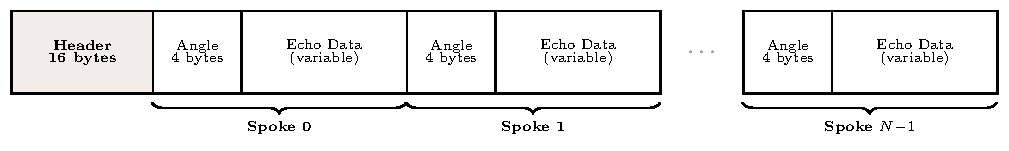
\includegraphics[width=\textwidth]{figures/new_figs/fig_sweep_structure.pdf}
\caption{Echo packet structure. A 16-byte header is followed by one or more spokes, each containing an angle sub-header and variable-length echo data.}
\label{fig:sweep}
\end{figure}

The radar completes 8{,}192 spokes per full $360\degree$ rotation. A single packet does not contain an entire rotation. Instead, spokes arrive across many packets over the course of one antenna revolution. The host software detects that a full rotation has completed when the azimuth value of a newly received spoke drops by more than 1{,}000 ticks compared to the previous spoke, indicating a wrap-around past zero.

After decoding, every spoke produces a fixed-length array of range bins. Each range bin represents the echo intensity at a specific distance from the radar along that spoke's azimuth. The number of range bins per spoke is typically 868, though this value varies with the radar's range setting and is specified in the packet header.


%==============================================================================
\section{Header}
\label{sec:header}
%==============================================================================

Every echo packet begins with a 16-byte header. The header contains packet sequencing information, a timestamp, and metadata fields that the decoder needs to interpret the spoke data that follows.

\begin{figure}[H]
\centering
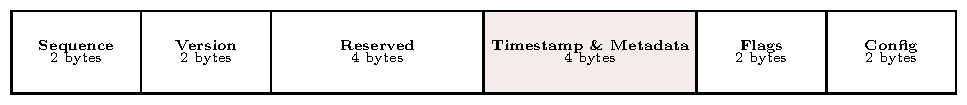
\includegraphics[width=\textwidth]{figures/new_figs/fig_header_fields.pdf}
\caption{The six fields of the 16-byte echo packet header.}
\label{fig:header}
\end{figure}

All multi-byte fields in the header use big-endian byte ordering. This is in contrast to the spoke sub-headers, which use little-endian ordering (see Section~\ref{sec:spoke}).

\begin{table}[H]
\centering
\caption{Echo packet header fields.}
\label{tab:header}
\begin{tabular}{@{}rrlp{7cm}@{}}
\toprule
\textbf{Offset} & \textbf{Size} & \textbf{Field} & \textbf{Description} \\
\midrule
0--1   & 2 bytes & Sequence  & Packet counter (u16 BE). Increments with each packet. Used for ordering and detecting packet loss. \\
2--3   & 2 bytes & Version   & Protocol version (u16 BE). Always \texttt{0x0001}. \\
4--7   & 4 bytes & Reserved  & Always \texttt{0x00000000}. Unused padding. \\
8--11  & 4 bytes & Timestamp \& Metadata & Radar clock timestamp (u32 BE). Also contains three metadata fields packed at the bit level (see Section~\ref{sec:metadata}). \\
12--13 & 2 bytes & Flags     & Always \texttt{0x1500}. Purpose not fully determined. \\
14--15 & 2 bytes & Config    & Always \texttt{0xF009}. Purpose not fully determined. \\
\bottomrule
\end{tabular}
\end{table}

Most header fields are static across all observed packets. The Sequence and Timestamp fields are the only values that change per packet. The Version, Reserved, Flags, and Config fields have been observed at fixed values across all range settings, scan speeds, and operating modes.

The minimum valid packet size is 20 bytes: the 16-byte header plus at least one 4-byte spoke sub-header. The critical information for decoding echo data is contained in bytes 8--11, described in the next section.


%==============================================================================
\section{Metadata (Bytes 8--11)}
\label{sec:metadata}
%==============================================================================

Bytes 8 through 11 of the header serve a dual purpose. The echo header parser reads them as a single 32-bit big-endian timestamp representing the radar's internal clock value. Simultaneously, the metadata parser inspects bytes 9, 10, and 11 individually to extract three fields that control how the spoke data is decoded.

\begin{figure}[H]
\centering
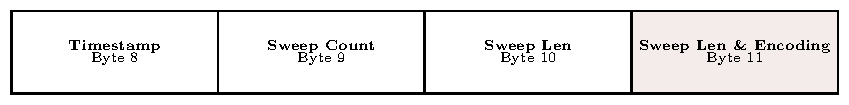
\includegraphics[width=\textwidth]{figures/new_figs/fig_metadata_bytes.pdf}
\caption{The four bytes of the timestamp and metadata region. Each byte carries a specific metadata field.}
\label{fig:metadata}
\end{figure}

\subsection{Byte 8: Timestamp}

Byte 8 is the high byte of the 32-bit radar clock timestamp. It contains no metadata fields. Its value changes with each packet as the radar clock advances.

\subsection{Byte 9: Sweep Count}

Byte 9 encodes the sweep count, which specifies how many spokes are packed into this packet. The sweep count occupies the upper 7 bits of the byte (bits 7 through 1). Bit 0 is unused.

\begin{align}
\texttt{sweep\_count} &= \texttt{data[9]} \gg 1
\end{align}

The sweep count can range from 0 to 127, though typical values vary with the radar's scan speed and range setting. The decoder uses this value to know how many spoke sub-headers and echo data blocks to expect after the header.

\subsection{Byte 10: Sweep Length (Low Byte)}

Byte 10 contains the low 8 bits of the sweep length. The sweep length specifies how many range bins each spoke will contain after decoding. This is the first half of an 11-bit value; the remaining 3 bits are in byte 11.

\subsection{Byte 11: Sweep Length (High Bits) and Encoding}

Byte 11 contains three fields packed into a single byte. This is the most densely packed byte in the header.

\begin{figure}[H]
\centering
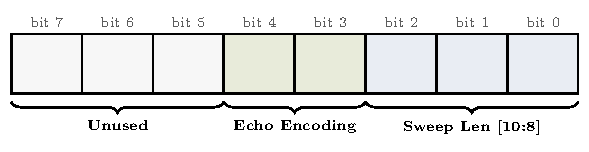
\includegraphics[width=0.8\textwidth]{figures/new_figs/fig_byte11_zoom.pdf}
\caption{Bit-level layout of byte 11, showing three packed fields.}
\label{fig:byte11}
\end{figure}

The three fields are extracted as follows.

\textit{Bits 7:5} (top 3 bits) are unused. They have been observed as zero across all captured packets.

\textit{Bits 4:3} (middle 2 bits) specify the echo encoding type. This 2-bit field selects one of four compression schemes that the radar has applied to the echo data in this packet. The four encoding types are described in detail in Section~\ref{sec:encoding}.

\begin{align}
\texttt{encoding} &= (\texttt{data[11]} \mathbin{\&} \texttt{0x18}) \gg 3
\end{align}

\textit{Bits 2:0} (bottom 3 bits) are the high 3 bits of the sweep length. Combined with byte 10, they form the complete 11-bit sweep length value.

\begin{align}
\texttt{sweep\_len} &= ((\texttt{data[11]} \mathbin{\&} \texttt{0x07}) \ll 8) \mathbin{|} \texttt{data[10]}
\end{align}

The sweep length is an 11-bit unsigned integer with a theoretical range of 0 to 2{,}047. The typical observed value is 868 range bins, though this varies with the radar's range setting.

\subsection{Worked Example}

Consider bytes 8--11 with values \texttt{[0xAB, 0x0A, 0x64, 0x0B]}.

Byte 9 is \texttt{0x0A}. The sweep count is $\texttt{0x0A} \gg 1 = 5$, so this packet contains 5 spokes.

Byte 10 is \texttt{0x64}, which is 100 in decimal. This is the low byte of the sweep length.

Byte 11 is \texttt{0x0B} (\texttt{0b00001011}). The encoding field is $(\texttt{0x0B} \mathbin{\&} \texttt{0x18}) \gg 3 = (\texttt{0x08}) \gg 3 = 1$, selecting Encoding 1 (repeating). The sweep length high bits are $\texttt{0x0B} \mathbin{\&} \texttt{0x07} = 3$. The full sweep length is $(3 \ll 8) \mathbin{|} 100 = 768 + 100 = 868$ range bins.

This packet therefore contains 5 spokes, each decoding to 868 range bins, compressed using Encoding 1.


%==============================================================================
\section{Spoke Data}
\label{sec:spoke}
%==============================================================================

After the 16-byte header, the packet contains a sequence of spokes. The number of spokes is given by the sweep count field (Section~\ref{sec:metadata}). Each spoke consists of a fixed 4-byte angle sub-header followed by a variable-length block of encoded echo data.

\begin{figure}[H]
\centering
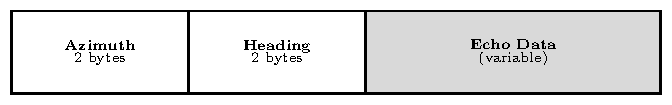
\includegraphics[width=0.7\textwidth]{figures/new_figs/fig_spoke_layout.pdf}
\caption{Structure of a single spoke: a 4-byte angle sub-header followed by variable-length echo data.}
\label{fig:spoke}
\end{figure}

\subsection{Angle Sub-Header}

The first 4 bytes of each spoke encode two angular measurements. Unlike the packet header, these fields use little-endian byte ordering.

\begin{table}[H]
\centering
\caption{Spoke angle sub-header fields.}
\label{tab:spoke}
\begin{tabular}{@{}rrlp{7cm}@{}}
\toprule
\textbf{Offset} & \textbf{Size} & \textbf{Field} & \textbf{Description} \\
\midrule
0--1 & 2 bytes & Azimuth & Antenna rotational position (u16 LE). Measured in ticks. \\
2--3 & 2 bytes & Heading & Compass bearing (u16 LE). Measured in ticks. \\
\bottomrule
\end{tabular}
\end{table}

Both fields use the same quantization: 8{,}192 ticks per full $360\degree$ rotation. This gives an angular resolution of $360 / 8{,}192 \approx 0.0439\degree$ per tick. The conversion from ticks to degrees is:

\begin{align}
\theta_{\text{deg}} &= \frac{\texttt{ticks}}{8{,}192} \times 360\degree
\end{align}

The azimuth field tracks the antenna's rotational position as it sweeps around. Azimuth values increment with each successive spoke and wrap from approximately 8{,}191 back toward 0 at the start of each new rotation.

The heading field independently tracks the compass bearing from the radar's internal compass sensor. This value is updated per spoke and allows the host to convert radar-relative azimuth angles to true geographic bearings.

\subsection{Echo Data}

The echo data block follows the 4-byte angle sub-header and contains the encoded echo amplitudes for this spoke. The length of this block on the wire is variable --- it depends on the encoding type and the data content. A spoke with many repeated values compresses to very few bytes, while a spoke with highly varied data may use nearly as many wire bytes as there are range bins.

After decoding, every spoke produces exactly \texttt{sweep\_len} range bins, regardless of how many wire bytes were consumed. Each decoded range bin is a single byte representing echo intensity.

After each spoke's echo data is consumed, the byte count is padded to the next 4-byte boundary:

\begin{align}
\texttt{consumed} &= (\texttt{n} + 3) \mathbin{\&} \lnot 3
\end{align}

This alignment ensures that each subsequent spoke's angle sub-header begins on a clean 4-byte boundary within the packet.

\subsection{Previous Spoke Buffer}

The decoder maintains a buffer called \texttt{prev\_spoke} that stores the most recently decoded spoke's raw (pre-display-conversion) values. This buffer is updated after every spoke and persists across both spokes within the same packet and across consecutive UDP packets. The previous spoke buffer is essential for Encoding 2 and Encoding 3, which reference the previous spoke's range bins during decoding (see Sections~\ref{subsec:enc2} and~\ref{subsec:enc3}).

\subsection{Display Conversion}

After decoding, every wire value undergoes a right-shift by 2 bits:

\begin{align}
\texttt{display} &= \texttt{wire} \gg 2
\end{align}

This converts 8-bit wire values (0--252) to 6-bit display values (0--63). The shift is applied uniformly regardless of encoding type. As discussed in Section~\ref{sec:encoding}, this shift has the convenient property of stripping the encoding control bits from the low bits of raw data values, producing a clean 0--63 intensity range for all four encodings.


%==============================================================================
\section{Echo Encoding}
\label{sec:encoding}
%==============================================================================

The radar applies one of four compression schemes to the echo data in each packet. The encoding type is specified by the 2-bit field in byte 11 of the header (see Section~\ref{sec:metadata}). All spokes within a single packet use the same encoding, but different packets within the same rotation may use different encodings.

The radar selects the encoding type adaptively based on the characteristics of the echo data at the time of transmission. The selection algorithm is implemented in the radar's firmware and has not been documented. In practice, Encoding 0 appears during sparse conditions, Encoding 1 during moderate spatial redundancy, and Encodings 2 and 3 during conditions where consecutive spokes share significant overlap.

All four encodings produce the same output: a fixed-length array of \texttt{sweep\_len} range bins. After decoding, the $\gg 2$ display conversion is applied uniformly. The control bits used by Encodings 1, 2, and 3 occupy the lowest 1 or 2 bits of each byte, which are exactly the bits discarded by the display shift. This is almost certainly by design.

\subsection{Encoding 0: No Compression}
\label{subsec:enc0}

Encoding 0 is the simplest scheme. Every byte in the echo data maps directly to one range bin with no compression.

\begin{figure}[H]
\centering
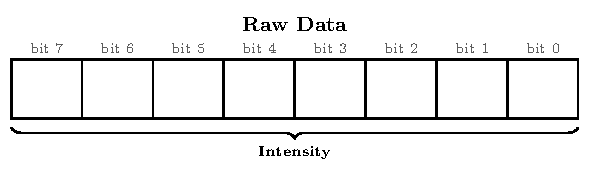
\includegraphics[width=0.6\textwidth]{figures/new_figs/fig_encoding0.pdf}
\caption{Encoding 0 byte layout. All 8 bits carry intensity data.}
\label{fig:enc0}
\end{figure}

The first \texttt{sweep\_len} bytes of the echo data are copied directly to form the decoded spoke. If fewer bytes are available than \texttt{sweep\_len}, the remaining bins are zero-padded. The consumed byte count is rounded up to the next 4-byte boundary.

Wire values span the full 0--252 range with no restrictions. After the $\gg 2$ display shift, this produces 64 distinct display levels (0--63). Encoding 0 provides no compression benefit but guarantees exact representation of every range bin.

\subsection{Encoding 1: Repeating}
\label{subsec:enc1}

Encoding 1 introduces run-length compression using a single control bit. Bit 0 (the least significant bit) of each byte determines whether the byte carries raw intensity data or a repeat instruction.

\begin{figure}[H]
\centering
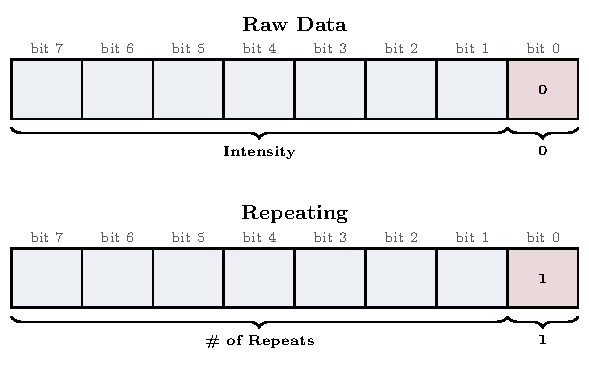
\includegraphics[width=0.6\textwidth]{figures/new_figs/fig_encoding1.pdf}
\caption{Encoding 1 byte layout. Bit 0 selects between raw data and repeating.}
\label{fig:enc1}
\end{figure}

When bit 0 is 0, the byte is a raw intensity value. The full byte is stored as the echo amplitude for the current range bin, and the decoder remembers this value as the ``current strength.'' Because bit 0 is always 0 for raw data bytes, the effective intensity values are restricted to even numbers: 0, 2, 4, \ldots, 252. This provides 127 distinct non-zero levels.

When bit 0 is 1, the byte is a repeat instruction. The decoder repeats the current strength value for a number of consecutive range bins. The repeat count is extracted from the upper 7 bits: $\texttt{count} = \texttt{byte} \gg 1$. A count value of 0 is treated as 128, allowing a single byte to fill up to 128 bins. The maximum explicitly encoded count is 127 (wire byte \texttt{0xFF}).

The current strength always refers to the most recently decoded raw data value, regardless of how many bins have been filled since it was set. Repeat instructions reference only this single value, making Encoding 1 a purely spatial compression scheme --- it exploits runs of identical intensity values along the spoke.

\subsubsection{Worked Example}

Consider the wire byte sequence \texttt{[0x3C, 0x07, 0x50, 0x05, 0x00]}.

\texttt{0x3C} has bit 0 = 0, so it is raw data with intensity 60. The current strength becomes 60. Bin 0 = 60.

\texttt{0x07} has bit 0 = 1, so it is a repeat. Count $= \texttt{0x07} \gg 1 = 3$. The current strength (60) is written into bins 1, 2, and 3.

\texttt{0x50} has bit 0 = 0, raw data with intensity 80. The current strength becomes 80. Bin 4 = 80.

\texttt{0x05} has bit 0 = 1, repeat. Count $= \texttt{0x05} \gg 1 = 2$. Bins 5 and 6 = 80.

\texttt{0x00} has bit 0 = 0, raw data with intensity 0. Bin 7 = 0.

The decoded spoke is \texttt{[60, 60, 60, 60, 80, 80, 80, 0]}, produced from 5 wire bytes --- a compression ratio of 5:8 in this example.

\subsection{Encoding 2: Copying from Previous Spoke}
\label{subsec:enc2}

Encoding 2 uses the same 1-bit control flag as Encoding 1, but the meaning of the repeat instruction changes. Instead of repeating the current strength, the decoder copies values from the previously decoded spoke at the corresponding range bin positions.

\begin{figure}[H]
\centering
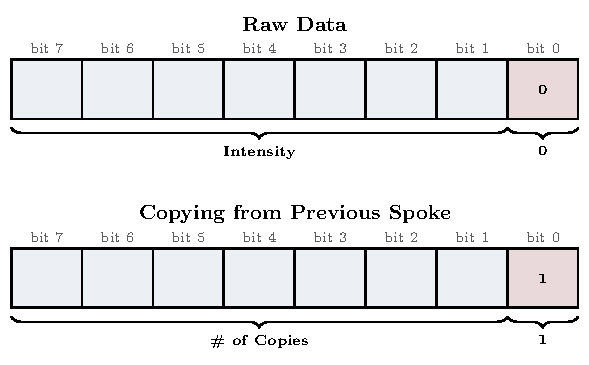
\includegraphics[width=0.6\textwidth]{figures/new_figs/fig_encoding2.pdf}
\caption{Encoding 2 byte layout. Bit 0 selects between raw data and copying from the previous spoke.}
\label{fig:enc2}
\end{figure}

When bit 0 is 0, the byte is raw data, identical to Encoding 1.

When bit 0 is 1, the decoder copies a number of consecutive range bins from the previous spoke. The copy starts at the current output index and reads from the same index in the previous spoke's data. The count formula is the same as Encoding 1: $\texttt{count} = \texttt{byte} \gg 1$, with 0 meaning 128.

This scheme exploits temporal redundancy. Consecutive radar spokes often observe similar echo patterns, particularly for stationary targets, coastlines, and consistent sea clutter. By encoding only the values that differ from the previous spoke, the radar can achieve significant compression for slowly-changing scenes.

The first spoke in a packet (\texttt{sweep\_idx == 0}) cannot use previous-spoke references because no prior spoke has been decoded in the current packet context. The decoder handles this by falling back to Encoding 1 behavior (repeating the current strength) for the first spoke, then using full Encoding 2 for subsequent spokes. The \texttt{prev\_spoke} buffer persists across UDP packets, so the temporal reference chain is maintained across packet boundaries.

\subsubsection{Worked Example}

Suppose the previous spoke contains \texttt{[60, 60, 80, 80, 40, 40, 20, 20]} and the wire bytes for the current spoke are \texttt{[0x50, 0x05, 0x3C, 0x07]}.

\texttt{0x50} has bit 0 = 0, raw data with intensity 80. Bin 0 = 80.

\texttt{0x05} has bit 0 = 1, copy from previous spoke. Count $= \texttt{0x05} \gg 1 = 2$. Copy bins 1 and 2 from the previous spoke: bin 1 = 60, bin 2 = 80.

\texttt{0x3C} has bit 0 = 0, raw data with intensity 60. Bin 3 = 60.

\texttt{0x07} has bit 0 = 1, copy from previous spoke. Count $= \texttt{0x07} \gg 1 = 3$. Copy bins 4, 5, and 6 from the previous spoke: bin 4 = 40, bin 5 = 40, bin 6 = 20.

The decoded spoke is \texttt{[80, 60, 80, 60, 40, 40, 20]}, mixing new raw values with temporally-referenced copies from the previous rotation.

\subsection{Encoding 3: Combined Repeating and Copying}
\label{subsec:enc3}

Encoding 3 is the most sophisticated scheme. It uses two control bits (bits 1:0) instead of one, providing three distinct operations within a single encoding. This combines the spatial compression of Encoding 1 with the temporal compression of Encoding 2.

\begin{figure}[H]
\centering
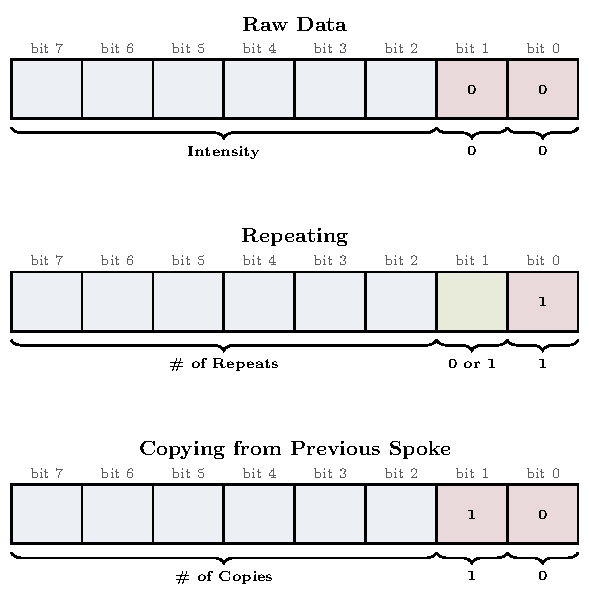
\includegraphics[width=0.6\textwidth]{figures/new_figs/fig_encoding3.pdf}
\caption{Encoding 3 byte layout. Bits 1:0 select between raw data, repeating, and copying from the previous spoke.}
\label{fig:enc3}
\end{figure}

When bits 1:0 are \texttt{00}, the byte is raw data. Since the bottom 2 bits are always zero for raw data bytes, the effective intensity values are restricted to multiples of 4: 0, 4, 8, \ldots, 252. This provides 64 distinct intensity levels, which maps exactly to the 0--63 display range after the $\gg 2$ conversion.

When bit 0 is 1 (bits 1:0 are \texttt{01} or \texttt{11}), the decoder repeats the current strength value, identical to Encoding 1. The count is extracted from the upper 6 bits: $\texttt{count} = \texttt{byte} \gg 2$. A count of 0 means 64. The maximum explicit count is 63.

When bits 1:0 are \texttt{10}, the decoder copies from the previous spoke at the corresponding range bin positions, identical to Encoding 2. The count formula is the same: $\texttt{count} = \texttt{byte} \gg 2$, with 0 meaning 64. During a copy operation, the internal strength variable is updated to the last copied value, so a subsequent repeat instruction will use the copied value rather than the previous raw data value.

The trade-off for combining both modes is reduced resolution. Only 6 bits remain for the count field (maximum 63, vs 127 in Encodings 1 and 2), and raw data values lose their bottom 2 bits (64 distinct levels, vs 127 in Encodings 1 and 2). However, the ability to mix spatial and temporal references within a single spoke provides the highest compression ratios for mixed scenes.

\subsubsection{Worked Example}

Suppose the previous spoke contains \texttt{[40, 40, 80, 80, 60, 60]} and the wire bytes are \texttt{[0x3C, 0x09, 0x0A, 0x50]}.

\texttt{0x3C} has bits 1:0 = \texttt{00}, raw data. Intensity $= \texttt{0x3C} = 60$. The current strength becomes 60. Bin 0 = 60.

\texttt{0x09} has bits 1:0 = \texttt{01}, bit 0 is 1, so this is a repeat. Count $= \texttt{0x09} \gg 2 = 2$. The current strength (60) is written into bins 1 and 2.

\texttt{0x0A} has bits 1:0 = \texttt{10}, copy from previous spoke. Count $= \texttt{0x0A} \gg 2 = 2$. Copy bins 3 and 4 from the previous spoke: bin 3 = 80, bin 4 = 60.

\texttt{0x50} has bits 1:0 = \texttt{00}, raw data. Intensity $= \texttt{0x50} = 80$. Bin 5 = 80.

The decoded spoke is \texttt{[60, 60, 60, 80, 60, 80]}, demonstrating all three operations in 4 wire bytes producing 6 range bins.

\subsection{Encoding Comparison}

\begin{table}[H]
\centering
\caption{Comparison of the four echo encoding schemes.}
\label{tab:encoding}
\begin{tabular}{@{}lcccc@{}}
\toprule
\textbf{Property} & \textbf{Enc 0} & \textbf{Enc 1} & \textbf{Enc 2} & \textbf{Enc 3} \\
\midrule
Control bits        & 0             & 1 (bit 0)      & 1 (bit 0)      & 2 (bits 1:0) \\
Intensity bits      & 8             & 7              & 7              & 6 \\
Raw data values     & 0--252        & even only      & even only      & multiples of 4 \\
Distinct levels     & 127           & 127            & 127            & 64 \\
Repeat last value   & ---           & yes            & ---            & yes \\
Copy from prev spoke & ---          & ---            & yes            & yes \\
Max count           & ---           & 128            & 128            & 64 \\
Compression type    & none          & spatial         & temporal       & both \\
\bottomrule
\end{tabular}
\end{table}

The $\gg 2$ display shift applied after decoding discards the bottom 2 bits of every wire value. This means the intensity restrictions imposed by the encoding control bits (even-only for Encodings 1 and 2, multiples-of-4 for Encoding 3) have no effect on the final display values. All four encodings produce the same 64-level (0--63) display range.


%==============================================================================
\section{Doppler Mode}
\label{sec:doppler}
%==============================================================================

The radar supports an optional Doppler target analysis mode that repurposes the most significant bit of each echo byte to indicate whether a target is moving. Doppler mode is activated via the \texttt{\$SEF} command (register \texttt{0xEF}) and can be set to one of three states: off (0), target analyzer (1), or rain mode (2).

\subsection{Echo Byte Layout}

When Doppler mode is active, the interpretation of each echo byte changes. In normal mode, all 8 bits encode intensity. In Doppler mode, bit 7 becomes a motion flag and the remaining 7 bits encode a reduced-range intensity value.

\begin{figure}[H]
\centering
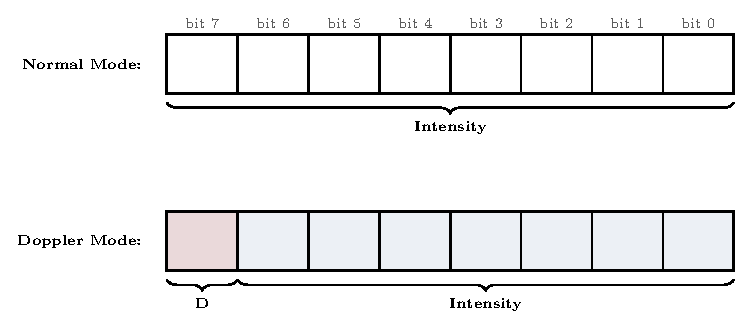
\includegraphics[width=0.6\textwidth]{figures/new_figs/fig_doppler_byte.pdf}
\caption{Echo byte layout in normal mode vs Doppler mode.}
\label{fig:doppler}
\end{figure}

In normal mode, the full byte represents echo intensity spanning 0 to 252. In Doppler mode, bit 7 serves as the D flag: 0 indicates a stationary target and 1 indicates a moving target. Bits 6 through 0 encode intensity compressed to 7 bits, spanning 0 to 126. The extraction operations are:

\begin{align}
D &= \texttt{byte} \mathbin{\&} \texttt{0x80} \\
\texttt{intensity} &= \texttt{byte} \mathbin{\&} \texttt{0x7F}
\end{align}

For example, the wire byte \texttt{0xC7} in Doppler mode decodes to $D = 1$ (moving target) with intensity $\texttt{0x47} = 71$.

\subsection{Status Field}

The Doppler mode status is communicated per spoke through a status field. Bit 8 of the status field (\texttt{0x100}) indicates whether Doppler data is present in the echo bytes. Bits 2:0 independently encode the pulse type.

\begin{table}[H]
\centering
\caption{Observed status field values.}
\label{tab:status}
\begin{tabular}{@{}rrl@{}}
\toprule
\textbf{Status} & \textbf{Binary} & \textbf{Meaning} \\
\midrule
1 (0x01)   & \texttt{0\_0000\_0001} & Normal echo, long pulse \\
4 (0x04)   & \texttt{0\_0000\_0100} & Normal echo, short pulse \\
257 (0x101) & \texttt{1\_0000\_0001} & Doppler echo, long pulse \\
260 (0x104) & \texttt{1\_0000\_0100} & Doppler echo, short pulse \\
\bottomrule
\end{tabular}
\end{table}

\subsection{Interaction with Encoding}

Doppler packing is applied by the radar hardware before the echo data is compressed. The encoding schemes described in Section~\ref{sec:encoding} operate on the raw 8-bit bytes without any knowledge of whether bit 7 carries a D flag or intensity data. The encoding control bits (bit 0 for Encodings 1 and 2, bits 1:0 for Encoding 3) occupy the low end of the byte and do not interfere with the D flag in bit 7.

This means the D flag passes through the entire encode/decode pipeline untouched. However, the current software implementation does not extract the D flag after decoding. The uniform $\gg 2$ display shift causes the D flag to bleed from bit 7 into bit 5 of the display value, adding 32 to the display intensity of moving targets. This produces a visual effect where moving targets appear brighter, but it is not an intentional Doppler visualization.

\subsection{Effective Bit Depths}

The combination of Doppler mode and encoding type determines the effective number of intensity bits available.

\begin{table}[H]
\centering
\caption{Effective intensity resolution across modes and encodings.}
\label{tab:bitdepth}
\begin{tabular}{@{}llcc@{}}
\toprule
\textbf{Mode} & \textbf{Encoding} & \textbf{Wire Intensity Bits} & \textbf{Display Levels} \\
\midrule
Normal  & 0       & 8 & 64 \\
Normal  & 1 / 2   & 7 & 64 \\
Normal  & 3       & 6 & 64 \\
Doppler & 0       & 7 & 32 (+32 if moving) \\
Doppler & 1 / 2   & 6 & 32 (+32 if moving) \\
Doppler & 3       & 5 & 32 (+32 if moving) \\
\bottomrule
\end{tabular}
\end{table}

In Doppler mode with Encoding 3, only 5 bits of intensity information remain in the wire byte. After the display shift, this yields 32 distinct intensity levels for stationary targets and a separate 32 levels (offset by +32) for moving targets.


%==============================================================================
\section{Dual-Pulse Interleaving}
\label{sec:dualpulse}
%==============================================================================

The radar alternates between two transmitter pulse types on consecutive spokes: a long pulse and a short pulse. This interleaving is a hardware characteristic of the solid-state transmitter and cannot be controlled by the host software. The pulse type for each spoke is encoded in bits 2:0 of the status field: a value of 1 indicates a long pulse, and a value of 4 indicates a short pulse.

\subsection{Long Pulse vs Short Pulse}

The two pulse types produce dramatically different intensity quantization.

Long-pulse spokes (status = 1) generate only 17 discrete intensity levels. The levels are not linearly spaced; the gaps between consecutive values grow with amplitude. The complete set of observed long-pulse values is:

\begin{lstlisting}
0, 8, 20, 28, 36, 44, 56, 64, 76, 88, 104, 120, 140, 164, 188, 220, 252
\end{lstlisting}

With 17 levels, the effective bit depth is approximately 4 bits ($\log_2 17 \approx 4.09$). The non-linear spacing provides finer resolution at low amplitudes, where distinguishing weak targets from noise is most important. The spacing between the lowest two non-zero levels is 12 (from 8 to 20), while the spacing between the highest two is 32 (from 220 to 252).

Short-pulse spokes (status = 4) produce 130 to 240 unique intensity values, depending on the Rez Boost setting. This provides near-continuous coverage of the 0--252 wire range, yielding an effective bit depth approaching 8 bits. Short pulses transmit less energy and therefore have reduced detection range, but provide much finer amplitude resolution.

\subsection{Range Dependence}

The ratio of long-pulse to short-pulse spokes varies with the radar's range setting. At short ranges, the radar uses a roughly equal mix of both pulse types. As the range increases, long-pulse spokes dominate because the additional transmit energy is needed to detect targets at greater distances.

\begin{table}[H]
\centering
\caption{Observed long/short pulse ratio by range setting.}
\label{tab:pulseratio}
\begin{tabular}{@{}llcc@{}}
\toprule
\textbf{Range Index} & \textbf{Distance} & \textbf{Long \%} & \textbf{Short \%} \\
\midrule
21    & 1/16 NM & 50\%   & 50\% \\
0     & 1/8 NM  & 50\%   & 50\% \\
3     & 3/4 NM  & 50\%   & 50\% \\
6     & 2 NM    & 51\%   & 49\% \\
9     & 6 NM    & 69\%   & 31\% \\
12    & 16 NM   & 99.9\% & 0.1\% \\
15    & 48 NM   & 99.9\% & 0.1\% \\
\bottomrule
\end{tabular}
\end{table}

At ranges beyond 16 NM, the radar produces almost exclusively long-pulse spokes, meaning the effective intensity resolution drops to approximately 17 levels for the majority of spokes.

\subsection{Rez Boost Effect}

Rez Boost (bearing resolution enhancement, register \texttt{\$SEE}) provides four levels: off (0), low (1), medium (2), and high (3). Increasing the Rez Boost level shifts the pulse ratio toward more short-pulse spokes and increases the number of unique intensity levels in short-pulse data.

\begin{table}[H]
\centering
\caption{Effect of Rez Boost on pulse ratio and short-pulse resolution.}
\label{tab:rezboost}
\begin{tabular}{@{}lccc@{}}
\toprule
\textbf{Rez Boost} & \textbf{Long \%} & \textbf{Short \%} & \textbf{Short Pulse Levels} \\
\midrule
Off (0)    & 81\% & 19\% & $\sim$130 \\
Low (1)    & 37\% & 63\% & $\sim$210 \\
Medium (2) & 39\% & 61\% & $\sim$240 \\
High (3)   & 36\% & 64\% & $\sim$240 \\
\bottomrule
\end{tabular}
\end{table}

With Rez Boost disabled, the radar produces predominantly long-pulse spokes (81\%), resulting in coarse 17-level quantization for most of the scan. Enabling Rez Boost at any level flips this ratio, producing roughly twice as many short-pulse spokes as long-pulse spokes. The difference between Low, Medium, and High settings is primarily in the number of unique intensity values: Low yields approximately 210 levels per short-pulse spoke, while Medium and High yield approximately 240.

\subsection{Current Implementation}

The current software implementation does not distinguish between long-pulse and short-pulse spokes. The status field (1 vs 4) is present in each spoke's data but is not extracted or stored in the \texttt{Spoke} structure. All spokes undergo the same decoding and display conversion regardless of pulse type. The 17-level quantization of long-pulse spokes and the fine quantization of short-pulse spokes are both mapped through the same $\gg 2$ display shift without any pulse-type-specific processing.


%==============================================================================
\section{Comparison to Other Marine Radars}
\label{sec:comparison}
%==============================================================================

The Furuno DRS4D-NXT echo protocol can be understood in context by comparing it to other consumer marine radar systems. The following data is drawn from community reverse-engineering efforts, primarily the OpenCPN \texttt{radar\_pi} plugin and the \texttt{mayara-server} project. Competitor specifications should be treated as approximate.

\subsection{Echo Transport and Spoke Format}

All systems surveyed use UDP over Ethernet for echo data, with the exception of the Raymarine Quantum which can also operate over Wi-Fi. The Furuno is unique in using TCP with ASCII-formatted commands for radar control, while all other brands use binary UDP commands.

\begin{table}[H]
\centering
\caption{Echo transport and spoke format comparison.}
\label{tab:compare-transport}
\begin{tabular}{@{}lcccc@{}}
\toprule
\textbf{Property} & \textbf{Furuno NXT} & \textbf{Navico HALO} & \textbf{Garmin xHD} & \textbf{Raymarine HD} \\
\midrule
Transport        & UDP multicast   & UDP multicast   & UDP multicast  & UDP multicast \\
Spokes/rotation  & 8{,}192         & 2{,}048         & 1{,}440        & 2{,}048 \\
Range bins/spoke & 883             & 1{,}024         & 705            & 1{,}024 \\
Spokes/packet    & $\sim$8         & 32              & 1              & variable \\
Angular res.     & 0.044\textdegree & 0.176\textdegree & 0.25\textdegree & 0.176\textdegree \\
\bottomrule
\end{tabular}
\end{table}

The Furuno's 8{,}192-spoke resolution is four times finer than Navico and Raymarine, and nearly six times finer than Garmin xHD. This is the highest angular resolution among consumer marine radars.

\subsection{Bit Depth and Encoding}

The approaches to echo amplitude encoding vary significantly across manufacturers.

\begin{table}[H]
\centering
\caption{Bit depth and compression comparison.}
\label{tab:compare-encoding}
\begin{tabular}{@{}lcccc@{}}
\toprule
\textbf{Property} & \textbf{Furuno NXT} & \textbf{Navico HALO} & \textbf{Garmin xHD} & \textbf{Raymarine HD} \\
\midrule
Bit depth          & 6 effective    & 4              & 8              & 8 \\
Intensity levels   & 64             & 16             & 256            & 256 \\
Compression        & 4 adaptive     & none           & none           & RLE \\
Encoding modes     & raw, RLE,      & raw nibbles    & raw bytes      & escape-byte \\
                   & delta, combined &                &                & RLE \\
\bottomrule
\end{tabular}
\end{table}

Navico packs two 4-bit samples per byte with no compression, yielding only 16 intensity levels but very simple decoding. Garmin xHD uses full 8-bit samples with no compression. Raymarine uses a straightforward RLE scheme with a dedicated escape byte (\texttt{0x5C}): when the decoder encounters this byte, the next byte is a repeat count and the byte after that is the value to repeat. This approach does not sacrifice any intensity bits but requires a full 3-byte sequence for each run, making it less space-efficient than Furuno's flag-bit approach.

The Furuno system is unique in offering four encoding modes selected adaptively per packet. The temporal delta encoding (Encoding 2) and combined mode (Encoding 3) have no equivalent in any other surveyed radar protocol. These modes exploit the similarity between consecutive spokes, a compression strategy that other manufacturers do not implement at the protocol level.

\subsection{Doppler}

Doppler target detection is available on only two of the surveyed platforms.

The Navico HALO implements Doppler through its VelocityTrack feature. When active, the 4-bit nibble values \texttt{0xF} and \texttt{0xE} take on special meaning: \texttt{0xF} indicates an approaching target and \texttt{0xE} indicates a receding target. No velocity magnitude is transmitted; the radar applies a configurable speed threshold internally and reports only a binary approaching/receding classification per range bin.

The Furuno DRS4D-NXT uses bit 7 of each echo byte as a D flag (0 = stationary, 1 = moving) when Doppler mode is active. Like Navico, this is a binary indicator rather than a velocity measurement. The key difference is that the Furuno D flag is embedded in the same byte as the intensity data, reducing intensity resolution from 8 to 7 bits, whereas Navico reserves specific nibble values from the existing 4-bit space.

Garmin and Raymarine HD do not support Doppler in their echo protocols. The Raymarine Quantum 2 has Doppler hardware, but the protocol encoding has not been documented.

\subsection{Summary}

The Furuno DRS4D-NXT protocol trades encoding complexity for flexibility. Its four adaptive compression modes, temporal spoke referencing, and integrated Doppler flag represent the most sophisticated echo encoding among consumer marine radars. The trade-off is a more complex decoder and a lower effective bit depth (6 bits, or 64 intensity levels) compared to the 8-bit raw data used by Garmin and Raymarine. However, the Furuno's angular resolution is unmatched, and its compression allows efficient bandwidth use despite streaming four times as many spokes per rotation as competing systems.


%==============================================================================
\end{document}
%==============================================================================
